\section{Results}
\label{sec:results}

The three contributions were proposed together, but they are not reported together. Each is
measured first on its own, against the same baseline, labelled \emph{none} in the tables: our
method with every change switched off, which is upstream TDA run through our code path
(Section~\ref{sec:method}). Comparing a contribution to this baseline rather than to the
separately run TDA rows isolates that one change, since the two runs differ by nothing
else. Where a contribution fails, we say why, and where the diagnosis suggests a repair, we test
the repair before moving on. Only then are the surviving pieces compared against zero-shot CLIP
and TDA together (Section~\ref{sec:together}).

\subsection{Contribution 1: margin-based cache admission}
\label{sec:margin}

Table~\ref{tab:margin} compares margin admission alone -- margin on, fusion off, temperature
off -- with the baseline, per dataset, together with the fraction of test samples
the gate admitted to the positive cache.

\begin{table}[htbp]
\centering
\begin{tabular}{lrrrrr}
\toprule
Dataset & none acc. & margin acc. & none ECE & margin ECE & Admission rate \\
\midrule
DTD & 47.04 & 44.86 & 17.41 & 20.11 & 52.96 \\
Flowers102 & 69.79 & 67.19 & 6.51 & 8.63 & 65.69 \\
Pets & 88.74 & 88.42 & 2.48 & 2.53 & 81.90 \\
EuroSAT & 53.22 & 48.91 & 14.43 & 26.38 & 26.54 \\
Aircraft & 24.21 & 18.96 & 15.56 & 32.64 & 15.93 \\
Mean & 56.60 & 53.67 & 11.28 & 18.06 & 48.60 \\
\bottomrule
\end{tabular}
\caption{Margin admission against the TDA-equivalent baseline (\emph{none}, all flags off, run in the same sweep): accuracy and ECE (\%) per dataset, and the fraction of test samples the margin gate admitted to the cache.}
\label{tab:margin}
\end{table}


Margin admission loses on every dataset and on both metrics. Mean accuracy drops from 56.60\%
to 53.67\% and mean ECE rises from 11.28\% to 18.06\%. The per-dataset spread is the
informative part. The threshold is one global constant, $1.0$ on raw logits, deliberately not tuned per dataset, because fitting it to each test set's own margin
distribution would be test-set tuning. Since CLIP's logits are $100\times$ a cosine similarity,
a gap of 1.0 asks for a top-1/top-2 cosine difference of only 0.01, a quantity with no
dataset-independent meaning. The admission column shows what that costs: the gate admits 15.9\%
of samples on Aircraft and 81.9\% on Pets, and the rate is ordered by zero-shot CLIP's accuracy
on the dataset, not by its class count (Flowers102 has the most classes and the second-highest
rate; EuroSAT has the fewest and the second-lowest). Where CLIP already separates the classes,
margins are wide and the gate opens; where CLIP is lost, every class looks like every other,
margins collapse, and the gate closes. The damage is ordered the same way: Pets, at 81.9\%
admission, is a near no-op (ECE $+0.05$ points), while Aircraft, at 15.9\%, doubles its ECE.

Three things went wrong, and the admission rate explains only the first.

\begin{enumerate}
    \item \textbf{The threshold does not port across datasets.} A fixed logit gap means
        different things on 10 and 100 classes, so one constant is simultaneously too loose
        on Pets and far too strict on Aircraft and EuroSAT.
    \item \textbf{A starving cache is not a smaller cache; it is a biased one.} If the cache
        were merely thinner, predictions would drift toward plain CLIP and calibration toward
        CLIP's own 5\%. Instead ECE doubles. At 16\% admission, most classes have no cache
        entry at all: only the classes CLIP finds easy clear the threshold, so the cache fills
        with those classes and nothing else. A new image's nearest cached neighbours can then
        only ever vote for an easy class, whatever the image actually shows. The cache becomes
        a prior pulling every prediction toward the handful of classes CLIP was already
        confident about -- which flips correct predictions on the under-represented classes
        (the accuracy drop) and adds those votes confidently (the ECE rise). Pets, with 37
        classes and 82\% admission, keeps every class covered, and nothing happens.
    \item \textbf{It filters on the wrong signal.} The diagnosis was that confidently
        \emph{wrong} samples enter the cache. But a confidently wrong prediction has a large
        margin, exactly like a confidently right one. Margin and entropy both measure how loud
        CLIP is, and neither sees correctness, so the gate could never remove the samples it
        was designed to remove. It only removed near-ties -- and upstream TDA's per-class
        eviction by entropy was already removing those wherever a class saw enough traffic.
        The gate was redundant where it was harmless and biasing where it bit.
\end{enumerate}

We therefore drop margin admission. Every variant from here on has margin admission off, and
the positive cache is filled by upstream TDA's own unconditional rule.

\subsection{Contribution 2: probabilistic fusion}
\label{sec:fusion}

Table~\ref{tab:fusion} compares probabilistic fusion as proposed in Section~\ref{sec:method}
-- fusion on with $w = 0.5$, margin off, temperature off -- with the baseline.

\begin{table}[htbp]
\centering
\begin{tabular}{lrrrr}
\toprule
Dataset & none acc. & fusion acc. & none ECE & fusion ECE \\
\midrule
DTD & 47.04 & 45.80 & 17.41 & 17.69 \\
Flowers102 & 69.79 & 68.90 & 6.51 & 32.46 \\
Pets & 88.74 & 88.77 & 2.48 & 43.78 \\
EuroSAT & 53.22 & 50.12 & 14.43 & 19.62 \\
Aircraft & 24.21 & 24.42 & 15.56 & 9.16 \\
Mean & 56.60 & 55.60 & 11.28 & 24.54 \\
\bottomrule
\end{tabular}
\caption{Probabilistic fusion as proposed (ungated, $w = 0.5$) against the TDA-equivalent baseline (\texttt{none}): accuracy and ECE (\%) per dataset.}
\label{tab:fusion}
\end{table}


Fusion as proposed is the worst single change in the project: mean ECE rises from 11.28\% to
24.54\%, driven by Flowers102 (6.51\% $\rightarrow$ 32.46\%) and Pets (2.48\% $\rightarrow$
43.78\%). Accuracy moves little (mean 56.60\% $\rightarrow$ 55.60\%), so the cache is still
doing its job of choosing the class; what breaks is the confidence attached to the choice.

The mechanism is visible in Eq.~\eqref{eq:fusion} once the two inputs' scales are compared.
The cache logits, computed exactly as in upstream TDA, are per class a sum of a few
$\exp(-\beta(1 - \mathrm{affinity}))$ terms over the cached items of that class.
With at most three items per class and affinity a cosine in $[-1, 1]$, the largest cache logit
is about 2 and most classes score near zero. Softmaxed over 100 classes, that is a nearly flat
distribution whose top entry is around 7\%. CLIP's logits, by contrast, carry its learned logit
scale ($\approx 100$) and are sharply peaked, often above 90\%. A 50/50 average of a peaked
distribution and a flat one halves the peak. Fusion therefore caps top-1 probability near one
half on every sample, right or wrong alike -- it does not need the two sources to agree on a
wrong answer; it produces the effect unconditionally. ECE penalises underconfidence exactly as it
penalises overconfidence, so the cost scales with accuracy: on Pets the model is right 88.77\% of
the time and reports roughly 45\% confidence, a gap of about 44 points, which is the 43.78\% in
the table. Aircraft is the one dataset where fusion's ECE looks like an improvement (15.56\%
$\rightarrow$ 9.16\%), and it is not a correction: Aircraft's true accuracy (24\%) happens to sit
close to where the confidence ceiling landed, so the same ceiling that ruins Pets lands near the
truth there by accident.

\paragraph{Gating the fusion.}
The diagnosis says fusion fails because it runs on every sample, including the large majority
where CLIP already has a clear winner and the cache can only dilute it. On those samples the
cache cannot change the argmax either way, so the right move is to leave it out entirely:
additive TDA would only sharpen (the original overconfidence) and fusion would only dilute. The
cache has a real job on exactly one kind of sample -- a two-way tie, where it can break the tie,
which is where TDA's accuracy gain comes from -- and on a genuine tie a confidence near one half
is roughly honest. We therefore gate the fusion. Let $p = \sigma(z_{\text{clip}})$ and let
$p_{(1)} \geq p_{(2)}$ be its two largest entries. A sample is a \emph{two-way tie} when
\begin{equation}
    p_{(1)} - p_{(2)} < 0.2 \quad\text{and}\quad p_{(1)} + p_{(2)} > 0.6 .
    \label{eq:gate}
\end{equation}
The first condition is the close call; the second is what ``low entropy'' buys: a sample spread
thinly over many classes also has a small top-two gap, but there CLIP is confused rather than
torn, and the cache's vote is noise. On a tie the output is Eq.~\eqref{eq:fusion} with
$w = 0.5$; otherwise it is $\sigma(z_{\text{clip}})$, CLIP's own distribution (corrected by
TDA's negative cache, which is untouched throughout), with the positive cache not consulted.
Both thresholds are in probability space, so one global pair means the same thing on 10 and
100 classes -- the portability margin admission lacked -- and both were fixed a priori before
any run, not tuned. The gate is a separate switch, off by default, so every run above is
unaffected.

Table~\ref{tab:gate} compares gated fusion -- gate on, margin off, temperature off -- with
the same baseline.

\begin{table}[htbp]
\centering
\begin{tabular}{lrrrr}
\toprule
Dataset & none acc. & gate acc. & none ECE & gate ECE \\
\midrule
DTD & 47.04 & 45.69 & 17.41 & 6.24 \\
Flowers102 & 69.79 & 69.02 & 6.51 & 4.08 \\
Pets & 88.74 & 88.77 & 2.48 & 5.68 \\
EuroSAT & 53.22 & 47.30 & 14.43 & 3.56 \\
Aircraft & 24.21 & 24.27 & 15.56 & 3.48 \\
Mean & 56.60 & 55.01 & 11.28 & 4.61 \\
\bottomrule
\end{tabular}
\caption{Gated probabilistic fusion against the TDA-equivalent baseline (\texttt{none}): accuracy and ECE (\%) per dataset.}
\label{tab:gate}
\end{table}


The blow-up is gone. Flowers102 and Pets return to single-digit ECE, and gated fusion beats the
baseline's ECE on four of five datasets, by ten or more points on three of them (DTD 17.41\%
$\rightarrow$ 6.24\%, EuroSAT 14.43\% $\rightarrow$ 3.56\%, Aircraft 15.56\% $\rightarrow$
3.48\%). Mean ECE falls from 11.28\% to 4.61\%, which is below zero-shot CLIP's own 5.57\%
(Section~\ref{sec:together}): the method is better calibrated than the frozen model it started
from. Pets is the one loss (2.48\% $\rightarrow$ 5.68\%), on the dataset where TDA was already
nearly perfectly calibrated. The accuracy side is the cost. Gated fusion matches or fractionally
exceeds the baseline on Pets and Aircraft, gives up 0.77 points on Flowers102 and 1.35 on DTD,
and 5.92 on EuroSAT, where it returns more than half of TDA's eleven-point gain. TDA's flips on
EuroSAT happen on samples with a moderate margin, pushed over by that dataset's strong cache
weighting ($\alpha = 4$, $\beta = 8$); the gate, by construction, keeps the cache out of those.

The gate uses the same quantity margin admission used -- the gap between CLIP's top two
scores -- and the contrast between the two is the clearest finding in this section. Margin
admission applied it at storage time, to decide what the cache remembers, and threw information
away permanently and unevenly across classes. The gate applies it at prediction time, to decide
when the cache is consulted, and leaves every class represented. Same test, opposite purpose:
admission kept the clear winners and discarded the close calls, while the gate leaves the clear
winners alone and brings the cache in only on the close calls, which are the only samples where
the cache can change anything but confidence.

\subsection{Contribution 3: leave-one-out temperature scaling}
\label{sec:temperature}

Table~\ref{tab:temp} compares LOO temperature scaling alone -- temperature on, margin off,
fusion off -- with the baseline.

\begin{table}[htbp]
\centering
\begin{tabular}{lrrrr}
\toprule
Dataset & none acc. & temp acc. & none ECE & temp ECE \\
\midrule
DTD & 47.04 & 47.04 & 17.41 & 4.68 \\
Flowers102 & 69.79 & 69.79 & 6.51 & 4.85 \\
Pets & 88.74 & 88.74 & 2.48 & 15.54 \\
EuroSAT & 53.22 & 53.22 & 14.43 & 13.43 \\
Aircraft & 24.21 & 24.21 & 15.56 & 4.21 \\
Mean & 56.60 & 56.60 & 11.28 & 8.54 \\
\bottomrule
\end{tabular}
\caption{LOO temperature scaling against the TDA-equivalent baseline (\emph{none}): accuracy and ECE (\%) per dataset. Accuracy is identical by construction.}
\label{tab:temp}
\end{table}


Accuracy is identical on every dataset, to 0.00 points. This is not a coincidence but a
structural guarantee: temperature scaling is a monotonic rescaling of the logits and cannot
change an argmax, so any difference would itself be a bug. On calibration it is a real but not
uniform improvement. Mean ECE falls from 11.28\% to 8.54\%, with large gains where the baseline
was badly overconfident (DTD 17.41\% $\rightarrow$ 4.68\%, Aircraft 15.56\% $\rightarrow$
4.21\%) and small ones on EuroSAT and Flowers102. On Pets it is a clear reversal: 2.48\%
$\rightarrow$ 15.54\%.

The Pets failure has a simple cause. The search has no stopping rule. It always moves mean
confidence toward the label-free accuracy estimate $\hat{a}$, whether or not the model was
already honest, so where TDA was already calibrated the only thing it can do is damage. And
$\hat{a}$ is biased low on fine-grained data: the estimate is leave-one-out nearest-neighbour
agreement inside the cache, and on Pets a cached Birman's nearest cached neighbour is often a
Ragdoll even when both pseudo-labels are correct, so the agreement rate sits well below the
true accuracy. The search reads that as ``accuracy is lower than confidence'' and smooths a model
that did not need it. The smoothing-only grid floor at $T = 1.0$ (Section~\ref{sec:method})
cannot help here; it only prevents the opposite mistake.

\subsection{Putting it together}
\label{sec:together}

Table~\ref{tab:main} compares the five headline methods on all five datasets: zero-shot CLIP
(CLIP), TDA, and three variants of our method -- gated fusion alone (Gate), LOO temperature
alone (Temp), and the two together (Gate+Temp). Margin admission is off in all three.

\begin{table}[htbp]
\centering
\begin{tabular}{lrrrrrrrrrr}
\toprule
 & \multicolumn{5}{c}{Accuracy} & \multicolumn{5}{c}{ECE} \\
\cmidrule(lr){2-6}\cmidrule(lr){7-11}
 & CLIP & TDA & Gate+Temp & Gate & Temp & CLIP & TDA & Gate+Temp & Gate & Temp \\
\midrule
DTD & 44.39 & 47.04 & 45.69 & 45.69 & 47.04 & 8.27 & 17.41 & 6.21 & 6.24 & 4.68 \\
Flowers102 & 67.32 & 69.91 & 69.02 & 69.02 & 69.79 & 2.63 & 6.39 & 5.89 & 4.08 & 4.85 \\
Pets & 88.20 & 88.77 & 88.77 & 88.77 & 88.74 & 4.37 & 2.52 & 13.90 & 5.68 & 15.54 \\
EuroSAT & 42.06 & 53.17 & 47.30 & 47.30 & 53.22 & 7.16 & 14.38 & 3.56 & 3.56 & 13.43 \\
Aircraft & 23.85 & 24.27 & 24.27 & 24.27 & 24.21 & 5.44 & 15.51 & 3.37 & 3.48 & 4.21 \\
Mean & 53.16 & 56.63 & 55.01 & 55.01 & 56.60 & 5.57 & 11.24 & 6.59 & 4.61 & 8.54 \\
\bottomrule
\end{tabular}
\caption{Top-1 accuracy and ECE (\%, 20 bins) on the five test splits. CLIP is zero-shot CLIP; Gate, Temp and Gate+Temp are our method with gated fusion, LOO temperature scaling, or both (margin admission off in all three). Mean is the unweighted mean over the five datasets.}
\label{tab:main}
\end{table}


Averaged over the five datasets, zero-shot CLIP reaches 53.16\% accuracy at 5.57\% ECE and
TDA 56.63\% at 11.24\%. Gated fusion alone reaches 55.01\% at 4.61\%: it keeps most of TDA's
accuracy gain over CLIP (1.85 of 3.47 points) while reporting better-calibrated confidence than
either. Figure~\ref{fig:scatter} shows the same comparison as a scatter: the target is a point
as far right as TDA and as far down as zero-shot CLIP, and the purple diamond sits below both
on three of the five datasets.

\begin{figure}[htbp]
    \centering
    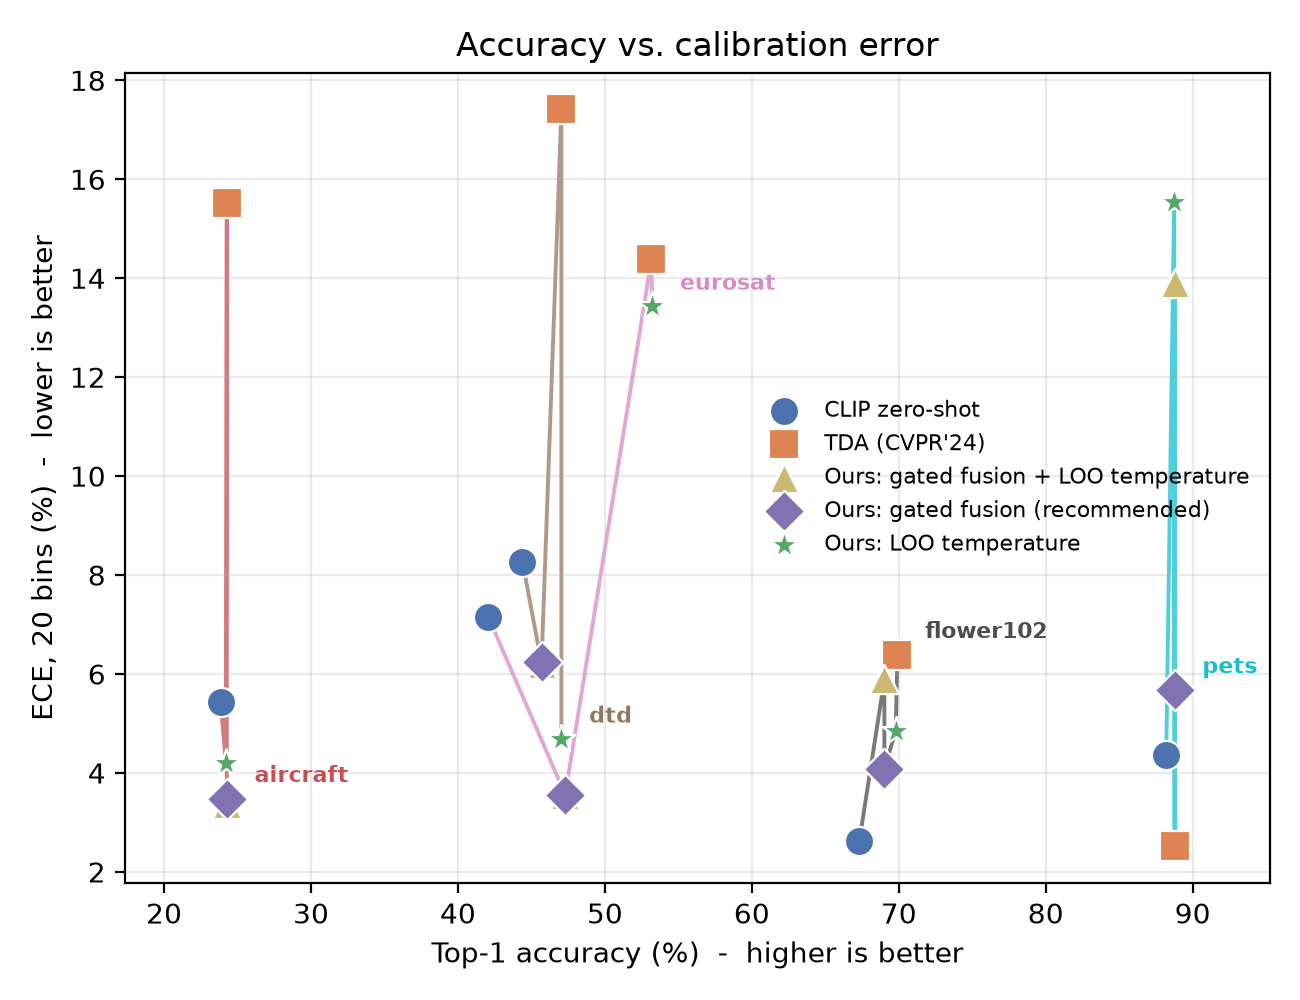
\includegraphics[width=0.75\textwidth]{accuracy_vs_ece.png}
    \caption{Accuracy vs.\ ECE on all five datasets for the five headline methods: zero-shot
    CLIP, TDA, and our method with gated fusion and LOO temperature together, gated fusion
    alone, and LOO temperature alone. Marker shape and colour identify the method (legend);
    each dataset's five points are joined by a line in that dataset's own colour, labelled at
    the line's right-hand end. Lines run left to right by accuracy and mark grouping only.}
    \label{fig:scatter}
\end{figure}

Table~\ref{tab:ablation-gate} is the ablation over the two surviving contributions: both on/off
combinations of gated fusion and LOO temperature, margin off, on all five datasets, 20 runs.

\begin{table}[htbp]
\centering
\begin{tabular}{lrr}
\toprule
 & Accuracy & ECE \\
\midrule
none: TDA-equivalent (both off) & 56.60 & 11.28 \\
gate: + gated fusion & 55.01 & 4.61 \\
temp: + LOO temperature & 56.60 & 8.54 \\
gate\_temp: + gated fusion + temperature & 55.01 & 6.59 \\
\bottomrule
\end{tabular}
\caption{Ablation with margin admission off: mean accuracy and ECE (\%) across the five datasets for gated fusion and LOO temperature.}
\label{tab:ablation-gate}
\end{table}


The two contributions do not stack. Adding temperature on top of the gate leaves accuracy
unchanged, as it must, and makes mean ECE worse (4.61\% $\rightarrow$ 6.59\%). The reason is
that both target the same thing. Temperature scaling was designed to undo the overconfidence
that TDA's cache manufactures; the gate removes that overconfidence at the source, by never
letting the cache sharpen a prediction CLIP had already made. What is left after the gate is
CLIP's own calibration, already around 5\%, and the label-free estimate is not accurate enough
to improve on it. On EuroSAT and Aircraft the search wants to sharpen, the floor at $T = 1$
blocks it, and the search is a no-op on 99.9\% and 92.5\% of samples respectively; on Pets it
acts on every sample and in the wrong direction (5.68\% $\rightarrow$ 13.90\%), the same Pets
failure as in Section~\ref{sec:temperature}. We therefore recommend gated fusion alone.

Figure~\ref{fig:reliability} plots, per dataset, the reliability curve for each of the five
headline methods. The direction of each failure is visible directly: TDA's curves sit below the
identity line (stated confidence exceeds accuracy), the temperature-only curves sit above it on
Pets (confidence below accuracy), and gated fusion tracks the diagonal most closely on DTD,
EuroSAT and Aircraft.

\begin{figure}[htbp]
    \centering
    % Three panels per row. Two-per-row was tried and reverted: five square panels
    % in three rows exceed \textheight, and LaTeX responds by pushing the caption
    % and the last subcaption clean off the bottom of the paper ("Float too large
    % for page by 128pt"). On-page legibility is fixed in make_figures.py instead,
    % by shrinking the matplotlib canvas rather than enlarging the float. Slot six
    % holds the legend the five panels share.
    \begin{subfigure}[t]{0.32\textwidth}
        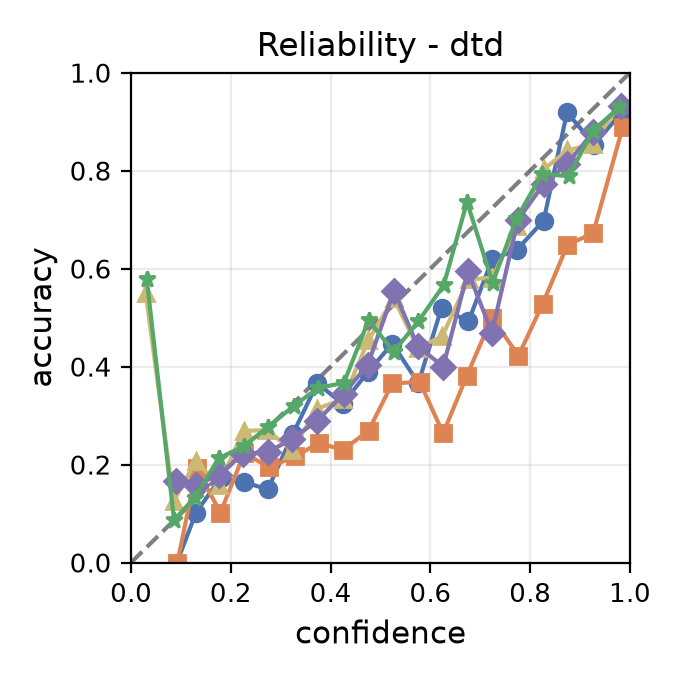
\includegraphics[width=\linewidth]{reliability_dtd.png}
        \caption{DTD}
    \end{subfigure}
    \begin{subfigure}[t]{0.32\textwidth}
        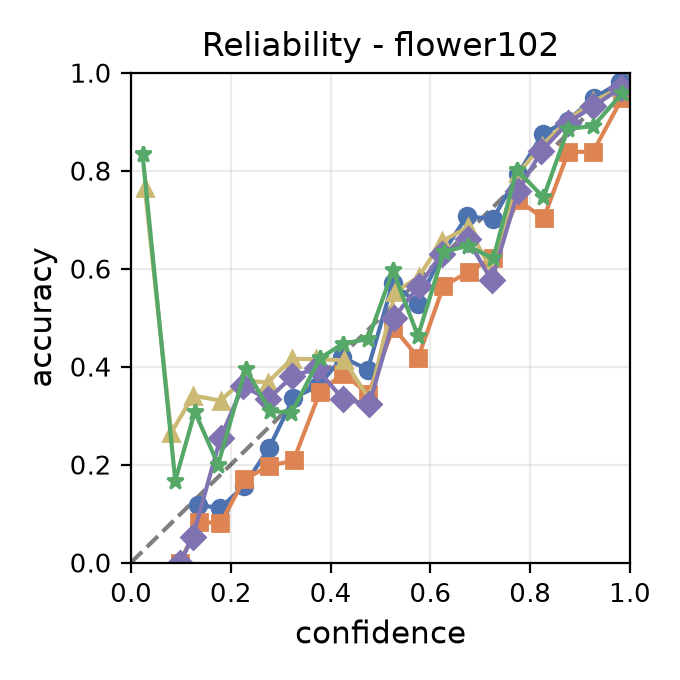
\includegraphics[width=\linewidth]{reliability_flower102.png}
        \caption{Flowers102}
    \end{subfigure}
    \begin{subfigure}[t]{0.32\textwidth}
        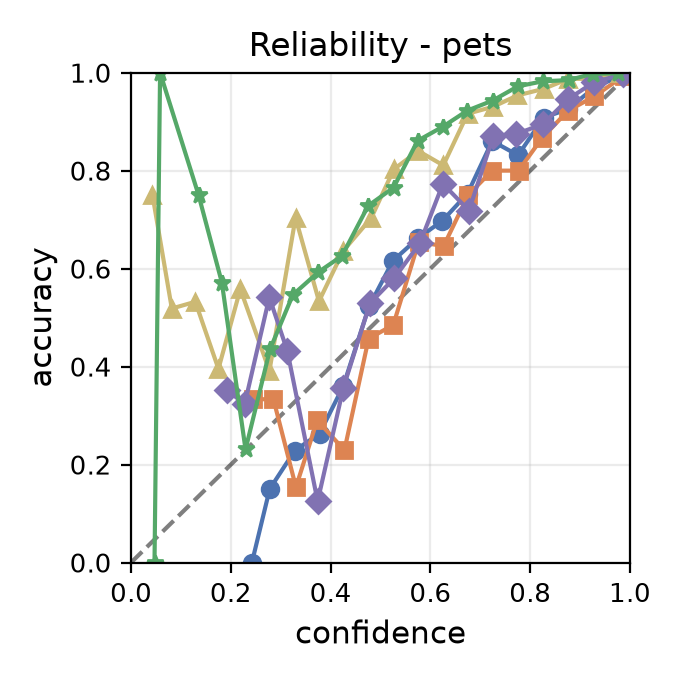
\includegraphics[width=\linewidth]{reliability_pets.png}
        \caption{Pets}
    \end{subfigure}\\[1ex]
    \begin{subfigure}[t]{0.32\textwidth}
        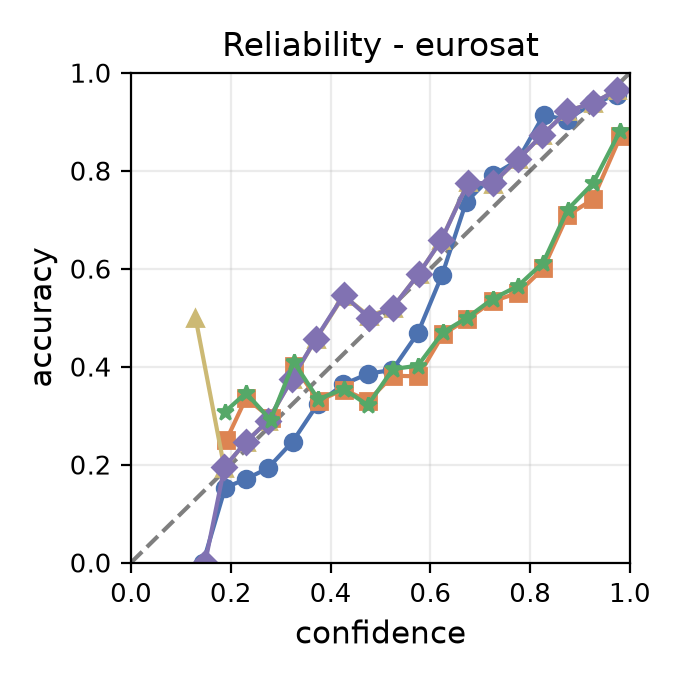
\includegraphics[width=\linewidth]{reliability_eurosat.png}
        \caption{EuroSAT}
    \end{subfigure}
    \begin{subfigure}[t]{0.32\textwidth}
        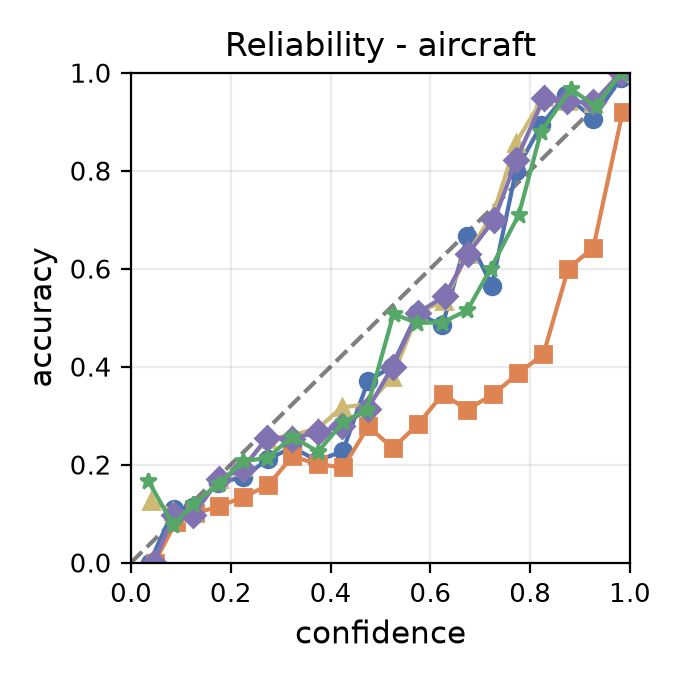
\includegraphics[width=\linewidth]{reliability_aircraft.png}
        \caption{Aircraft}
    \end{subfigure}
    % A minipage, not a subfigure: the legend is not a sixth panel and must not be
    % lettered (f) or counted in the figure's subcaptions.
    %
    % [b], not [t], and an explicit height. Given a height, minipage's [t] puts the
    % box *top* on the row's baseline -- which is the bottom edge of the panels
    % beside it, so the legend landed a full panel below the row. [b] puts the box
    % bottom there instead, so a box exactly one panel high (0.32\textwidth: the
    % panels are square) spans the row, and inner-pos c centres the legend in it.
    \begin{minipage}[b][0.32\textwidth][c]{0.32\textwidth}
        \centering
        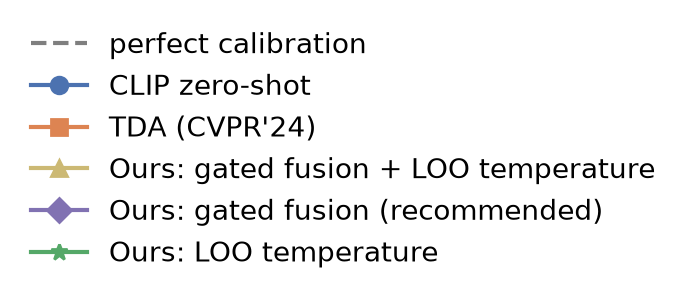
\includegraphics[width=\linewidth]{reliability_legend.png}
    \end{minipage}
    \caption{Reliability diagrams, all five datasets, for the same five methods as
    Figure~\ref{fig:scatter}: zero-shot CLIP, TDA, gated fusion + LOO temperature, gated
    fusion alone, and LOO temperature alone. All five panels share the legend at bottom right;
    a curve on the dashed identity line is perfectly calibrated.}
    \label{fig:reliability}
\end{figure}

\paragraph{The success criterion, counted honestly.}
The project's criterion was accuracy $\geq$ TDA \emph{and} ECE $<$ TDA on at least 3 of 5
datasets, against the TDA column of Table~\ref{tab:main}. Gated fusion meets
it on Aircraft only: it ties TDA's accuracy on Pets but loses on ECE there, and on DTD,
Flowers102 and EuroSAT it beats TDA's ECE by a wide margin while sitting below TDA's accuracy
by 1.35, 0.89 and 5.87 points. Temperature alone meets it on 2 of 5 (DTD and EuroSAT; on the
other three its accuracy is a few hundredths below the separately run TDA numbers, the
floating-point drift described in Section~\ref{sec:limitations}). No variant reaches 3 of 5.
What the method does deliver is different from what the criterion asks for: it trades a small
part of TDA's accuracy gain for calibration better than the frozen model's, and it does so
without labels, without training, and with one extra comparison per sample.

\subsection{Limitations}
\label{sec:limitations}

Every number here is one seed, one backbone (\texttt{ViT-B/16}) and five datasets. That is
enough to establish that margin admission and ungated fusion fail, that the gate repairs fusion,
and that temperature does not stack on it; it is not enough to claim the gate's margins hold
universally, and the smaller effects (the one-point EuroSAT ECE change under temperature, the
sub-point accuracy gaps on Pets and Aircraft) are within what a different stream order could
plausibly move. The gate's two thresholds were fixed a priori and have been tested on nothing
but these five datasets. Its accuracy cost on EuroSAT is real and would need a dataset-aware
gap -- which is to say, tuning -- to recover. The LOO estimate is only as good as the cache it
reads, and it is biased low on fine-grained data, which is what breaks temperature scaling on
Pets. Finally, the baseline and the separately run TDA rows differ by
0--4 flipped predictions per dataset out of 1{,}692--8{,}100: upstream TDA accumulates
its final logits in fp16 while our implementation upcasts to fp32 before its final step, and at
CLIP's logit magnitudes that rounding step is worth about one unit in the last place, enough to
flip a borderline argmax once every few hundred to few thousand samples. This is two orders of
magnitude below any effect discussed above, but it is why the two baselines are two distinct,
both-correct sets of numbers rather than duplicates.
